%Schemaless schema 
\chapter{Data Model}

%Entities
\section{Entities and their Relationships}

The first step for the development of the new JAQPOT Quattro
platform is to savy the essential entities of the project
and their relationships.
The ER sketch of JAQPOT Quattro is inspirited by the OpenTox
ontology and is concisely presented in the next figure.

\subsection{User}
JAQPOT stores some very basic information about users so as to
manage users' quota. Users have identifying information such as 
their email and name, and a list of limitations (if any) such 
as the maximum number of parallel tasks they can run on the system,
the maximum number of models they may store, datasets to create and
so on.

\subsection{Task and Error Report}
A task is identified by its ID. It has a status (running, queued,
cancelled, etc), percentage of completion, duration to complete (when
it has completed), URI of the result, corresponding HTTP status, 
and also points to the User who created it in the first place, 
as well as a creation timestamp. In case of an exceptional 
event, it links to an ErrorReport entity. This has an error code
(internal), HTTP status, debugging details, error message, 
actor (who is to blame for the exception), and an identifying ID.

\begin{figure}
 \centering
 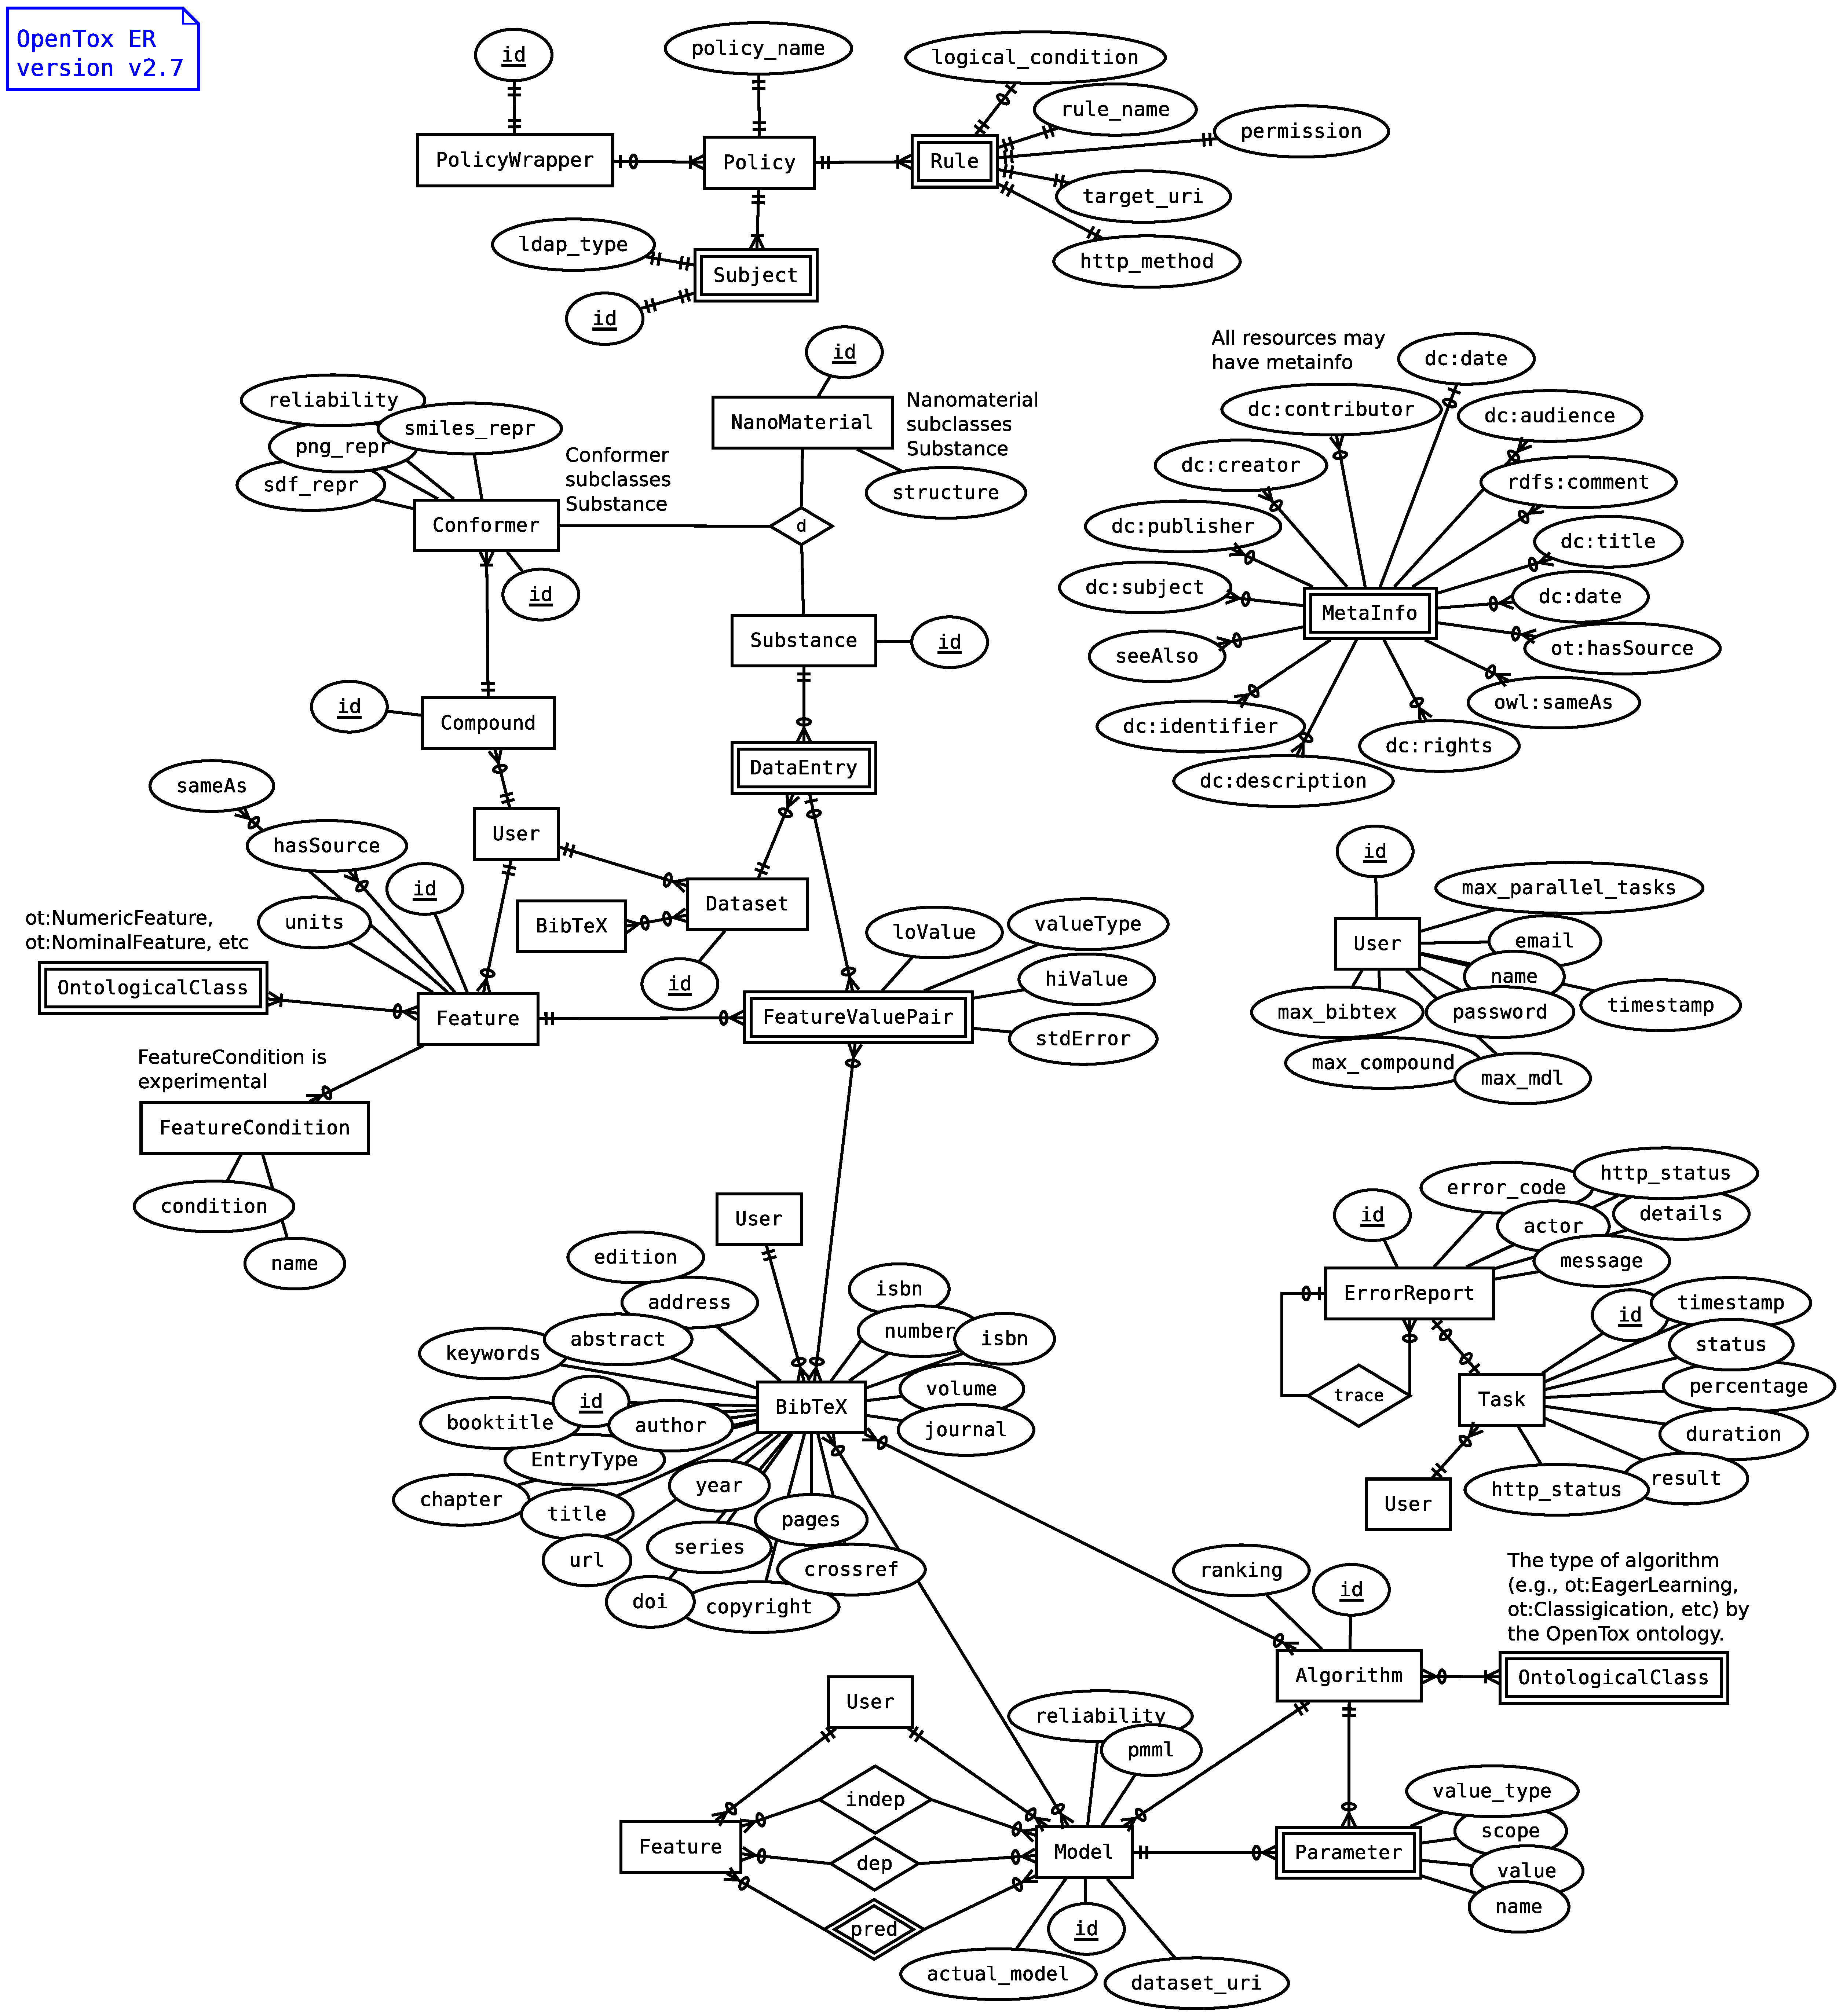
\includegraphics[keepaspectratio=true,width=0.99\textwidth]{figures/er}
\end{figure}

\subsection{Substance}
Substance is a central figure in JAQPOT: A Substance can be either a
chemical Conformer or a Nanomaterial, while in the future other classes
may be added (e.g., proteins, DNA, etc.). A Substance from JAQPOT's
perspective is (i) what identifies a \textit{row} in a \textit{dataset} for
training and (ii) input for prediction using a model.
Substances are abstract entitied. In particular, in the current version, they
are subclassed by the distinct classes \texttt{Nanomaterial} and \texttt{Conformer}.

\subsection{Conformer}
A Conformer is a chemical compound with a particular 3D configuration.
Chemical conformers are groupped together by the same \texttt{Compound}.
Conformers are characterized by their IDs and their various representations
(SMILES, SDF, InChI, etc).

\subsection{Nanomaterials}
A nanomaterial is a particular instance of a Substance. Nanomaterials'
structure is described by the NPO ontology (http://www.nano-ontology.org/).



\subsection{Feature}
Features are properties that can be assigned to substances. The type of
a feature is determined by a link to an ontological class. For instance
a feature can be \texttt{ot:NominalFeature} or \texttt{ot:NumericFeature}
etc. Different features may be groupped together via \texttt{FeatureCondition}s.
Features possess also an ontological characterisation that can be 
used to search for them. When the feature can be computed \textit{in silico}
its \texttt{hasSource} attribute
is a link to the algorithm or model that can be used to compute it.


\subsection{FeatureValuePair}
A \texttt{FeatureValuePair} is exactly what its name implies: 
an feature-value pair in the database
for a particular substance and a given feature.
A Feature value pair may be part of a \texttt{DataEntry} whic is 
the elementary component of a Dataset. This entity has a lower
and a higher bound (in case it is single-valued, by convention,
\texttt{loValue} stores the value and \texttt{hiValue} is set to 
\texttt{null}. It has a value type (numeric, double, integer, 
etc), an error estimation (\textit{e.g.}, \texttt{stdError}).


\subsection{DataEntry and Dataset}
A data entry is simply a \textit{row} in a dataset;
there is a single substance (chemical conformer or nanomaterial) to which
the DataEntry pertains to. A Dataset is chiefly a collection of 
DataEntry entities. 
\section{Querying requirements}



\noindent Here we present a list of queries that one will be expected 
to perform on the DB based on the REST API of OpenTox.

\noindent General remarks:
\begin{enumerate}
 \item Consistency on delete is not an important feature of Jaqpot.
 \item Other comments
\end{enumerate}


\subsection{Tasks and Error Reports}

\noindent Read operations:
\begin{enumerate}
 \item Get task representation by ID
 \item Get a list of task IDs:
    \begin{enumerate}
    \item from a given user
    \item with a given status (\textit{e.g.}, running)
    \end{enumerate}
 \item List all task IDs (paginated)
\end{enumerate}

\noindent Write operations:
\begin{enumerate}
 \item Write new task as \texttt{QUEUED} (default)
 \item Update the meta-data and/or status of a task
\end{enumerate}

\noindent Remarks:
\begin{enumerate}
 \item 	Here we have the most write and read intensive DB 
	operations. Tasks can well be stored in an independent 
	in-memory DB such as Redis. However, this would mean 
	that when we restart the server, all tasks will be lost. 
	Not sure this is the best choice. We can still store the 
	tasks in a document DB (e.g., CouchBase).
 \item 	In case of nested ErrorReport entities, children reports are 
        only fetched with their parents.
\end{enumerate}



\subsection{Model}

\noindent Read operations:
\begin{enumerate}
 \item Retrieve a model: Get model representation (metadata only -- 
       no need to load the actual model) given the ID of the model.
 \item Fetch only the actual model (binary object) but not the metadata. 
 \item List all models of a user
 \item List all models of an algorithm 
 \item List all models for a given keyword (facilitate searching in meta-data)
 \item Combinations of the two above (by user and algorithm)
 \item List all model IDs (paginated)
\end{enumerate}


\noindent Write operations:
\begin{enumerate}
 \item Register new model (all info)
 \item Update model to link to a new BibTeX
 \item Update the meta-data of a model (\textit{e.g.}, new title)
 \item Delete or disable model 
\end{enumerate}


\noindent Remarks:
\begin{enumerate}
 \item In models as well as in other resources, when retrieving data from the 
       DB there will never be the need to fetch the user data (only the ID 
       of the user is OK).
 \item Notice that the actual model (binary) and its metadata are never loaded simultaneously.
 \item In the OpenTox API one finds the method \texttt{GET /model/{id}/independent} 
       (and related methods), but there is not need to create very specialized 
       queries to serve these cases. If the model is stored as a document in the DB, 
       it can be retrieved as a whole and then we can pick only the information we are interested in.
\end{enumerate}





\subsection{User}

\noindent Read operations:
\begin{enumerate}
 \item List all user IDs
 \item Get the representation of a user by ID
 \item Get user's quota (part of the user representation actually)
\end{enumerate}


\noindent Write operations:
\begin{enumerate}
  \item Create new user
  \item Update user quota limits
  \item Delete user
\end{enumerate}



\subsection{BibTeX}

\noindent Read operations:
\begin{enumerate}
\item Get the full representation of a BibTeX entity
\item Search given a keyword
\item List all BibTeX entries
\end{enumerate}

\noindent Write operations:
\begin{enumerate}
 \item Create new BibTeX
 \item Update BibTeX
 \item Delete BibTeX
\end{enumerate}


\noindent Remarks:\\
BibTeX entities have really a lot of fields and it wouldn’t make sense 
to have indexes for every such field. In these cases, we can introduce simply 
a new keyword field that will be indexed and will do the job.


\subsection{Features}
\noindent Read operations
\begin{enumerate}
 \item Get representation of a feature by ID
 \item List features (not too important)
 \item Search features that are sameAs some other feature or feature category (ontology)
 \item Search for features by \texttt{hasSource}
 \item Search for features by their name or some keyword
\end{enumerate}
 

\noindent Write operations
\begin{enumerate}
 \item Create new feature
 \item Update a feature (replace)
 \item Delete feature
\end{enumerate}



\subsection{Compounds}

\noindent Read operations:
\begin{enumerate}
 \item List compound IDs (paginated)
\item  Fetch the representation of a compound ID
\item  Search for the ID of a compound: (i) according to a keyword (we can use ElasticSearch) 
       and/or (ii) the is \texttt{sameAs} some other feature or feature category from an ontology
\item  Fetch a compound along with some features [returns a dataset]. 
   The corresponding API method is \texttt{GET /compound/\{cid\}/feature}
\item  Get all the conformers of a given compound
\end{enumerate}


\noindent Write operations:
\begin{enumerate}
\item Write a new compound in the DB
\item  Update compound
\item  Delete compound
\item  Add conformers to a given compound
\item  Update the representation of a conformer (using PUT)
\end{enumerate}


\noindent Remarks
\begin{enumerate}
\item  It is important to decide whether we will be saving every 
representation of the compound in the database, or whether the new 
representation will be calculated on the fly from what is found in the DB. 
\textit{e.g.}, A client uploads the compound ‘aspirin’ on jaqpot4 in SDF and 
creates a new resource, namely \texttt{/compound/123}. 
Then one needs to retrieve \texttt{/compound/123} is MOL format. 
Will this be generated on the fly? I guess this depends on how fast 
this conversion can be done. 
\item When retrieving datasets from the DB we do not need to 
retrieve any representation of the compound. All compounds appear as links in the dataset.
\end{enumerate}



\subsection{FeatureValuePair}

The only operation that is related to FeatureValuePair entities is the one implied by the API method 
\texttt{POST /compound/\{cid\}/feature?feature\_uri=\{feature\}\& value=\{value\}} 
where a new value is stored in the DB as a FeatureValuePair

\subsection{Dataset}

\noindent Read operations
\begin{enumerate}
 \item Get all dataset IDs (list, paginated)
\item  Fetch a dataset of given ID
\item  List all datasets (IDs) that have a property (\textit{e.g.}, 
   \texttt{created by user x} or \texttt{are annotated as \#jaqpot}). This can be simply done using ElasticSearch!
\item  Get all features and feature values of a given compound (also discussed in Section “Compound”)
\item  Merge datasets
\item  Add compounds to datasets (creates new dataset on the fly)
\item  Fetch a dataset and append a few features
\end{enumerate}


\noindent Write operations
\begin{enumerate}
\item  Create a new dataset (store all its values and the whole structure in the DB)
\item  Update a dataset (replace existing one)
\item Delete a dataset
\end{enumerate}

\noindent Remark: It seems we cannot store datasets in compact documents for many reasons. 
One reason is that whenever a feature-value pair entry is modified, this needs to be known to 
all datasets that use this value. \textit{e.g.}, if a client needs to modify the value of \texttt{molecular mass}
of \texttt{aspirin}, this needs to be updated in all datasets. 
Datasets are therefore collections of DataEntry entities.




\subsection{Algorithm}

There are certain cases that we need to store Algorithm entities
in the DB. Descriptor calculation algorithms (especially when they 
admit input parameters) may need to store new algorithm objects in the database. 
See http://opentox.org/
dev/apis/api-1.2/Algorithm\#section-7 for details. 
Algorithms are simply stored and retrieved as documents. Search is necessary only 
to return those algorithms that are sameAs some ontological category (need for one index). 
In detail we have:

\noindent Read operations
\begin{enumerate}
 \item List all algorithms
\item  Fetch algorithm by ID
\item  List algorithms that are sameAs a given ontological class
\item  List all algorithms generated by a user
\end{enumerate}

\noindent Write operations\\
Register a new algorithm

\subsection{Policy}

\noindent Read operations
\begin{enumerate}
 \item Fetch a policy of a given ID
\item  List all policies of a given user
\item  Search for a policy for a URI (allowed to the owner of the policy only)
\end{enumerate}


\noindent Write operations
\begin{enumerate}
\item  Register policy
\item  Update policy (replace)
\item  Delete policy
\end{enumerate}

\section{Database schema}
JAQPOT Quattro will make use of a document database, 
which is to a good extent schema-less. Here we discuss about 
the basic documents of JAQPOT Quattro and the indexes we need to 
introduce so as to maximize the performance of the 
search, insert and update operations defined previously.

The overall data schema refers to three databases:

\begin{enumerate}
 \item  A document database, in our case mongodb, that stores data in the form of documents. Most of JAQPOT’s resources are stored in this database,
\item  A relational database system, here mysql, that stores certain relations that have to do with datasets
\item  An ElasticSearch DB system that stores keyword-related data to facilitate the exploration of our domain.
\end{enumerate}

\subsection{Task and ErrorReport}

\textit{Example 1.} A completed task (note: duration is in milliseconds).

\begin{lstlisting}[language=json]
{ 
    "status":"COMPLETED", 
    "http_status":200, 
    "result": "http://opentox.ntua.gr:8080/model/234", 
    "duration":452, 
    "progress":[ 
        "data loaded", 
        "new resources have been created", 
        "now training the model", 
        "model training completed", 
        "result: OK" 
        ], 
    "creator":"guest@opentox.ntua.gr", 
    "time_created":"2015-12-01 14:04:45 CET" 
} 
\end{lstlisting}

\noindent \textit{Example 2.} A failed task with an error report in it:
\begin{lstlisting}[language=json]
{ 
    "status":"ERROR", 
    "http_status":400, 
    "duration":200, 
    "progress":[ 
        "data loaded", 
        "new resources have been created", 
        "now training the model", 
        "failed!" 
        ], 
    "creator":"guest@opentox.ntua.gr", 
    "time_created":"2015-12-01 14:04:45 CET", 
    "error_report":{ 
        "error_code":"XR243", 
        "actor":"client with IP 10.8.0.4", 
        "message":"Malformed input data", 
        "details":"Provide some details here to assist debugging", 
        "trace": { 
            "comment":"some other error report goes here if necessary" 
        } 
    } 
} 
\end{lstlisting}

\noindent \textit{Example 3.} A running task:
\begin{lstlisting}[language=json]
{ 
    "status":"RUNNING", 
    "percentage":57, 
    "http_status":202, 
    "progress":[ 
        "data loaded", 
        "new resources have been created", 
        "now training the model" 
        ], 
    "creator":"guest@opentox.ntua.gr", 
    "time_created":"2015-12-01 14:04:45 CET" 
} 
\end{lstlisting}

Notice that we do not assign IDs to the above documents since 
mongodb will create automatically a unique ID which is always 
denoted by \texttt{\_id}.

Indexes:
1. creator
2. status
3. (creator, status)

\begin{lstlisting}[language=json]
db.tasks.ensureIndex({"creator":1});
db.tasks.ensureIndex({"status":1});
db.tasks.ensureIndex({"creator":1, "status":1});
\end{lstlisting}

One can update the metadata of a task. 
See this example:
\begin{lstlisting}[language=json]
db.tasks.update( 
  { _id: ObjectId("54b454f8feee5a13a43f34f3") },  
  { $addToSet:  
     { "progress": "moved to step 4" } 
  } 
); 
\end{lstlisting}

All other update operations can be performed in a very standard way.

It is possible to fetch the data of a document from the DB without the data in a given field. For example, we can fetch a task without the progress information (here we assume we know the ID of the task):

\begin{lstlisting}[language=json]
db.tasks.find(
  {_id: ObjectId("54b454f8feee5a13a43f34f3")}, 
  {progress:0}
).pretty();
\end{lstlisting}

in some cases we may need to check only the status of a task (provided that we know its ID):
\begin{lstlisting}[language=json]
db.tasks.find(
  {_id: ObjectId("54b454f8feee5a13a43f34f3")}, 
  {status:1}
).pretty();
\end{lstlisting}

Remarks:
1. Tasks should be implemented as TTL (time-to-live) collections so that old tasks are garbage-collected.